\documentclass[times,specification,annotation]{itmo-student-thesis}

%% Опции пакета:
%% - specification - если есть, генерируется задание, иначе не генерируется
%% - annotation - если есть, генерируется аннотация, иначе не генерируется
%% - times - делает все шрифтом Times New Roman, собирается с помощью xelatex
%% - pscyr - делает все шрифтом Times New Roman, требует пакета pscyr.

%% Делает запятую в формулах более интеллектуальной, например:
%% $1,5x$ будет читаться как полтора икса, а не один запятая пять иксов.
%% Однако если написать $1, 5x$, то все будет как прежде.
\usepackage{icomma}

%% Один из пакетов, позволяющий делать таблицы на всю ширину текста.
\usepackage{tabularx}

\usepackage{longtable}

%% Данные пакеты необязательны к использованию в бакалаврских/магистерских
%% Они нужны для иллюстративных целей
%% Начало
\usepackage{tikz}
\usetikzlibrary{arrows}
\usepackage{filecontents}
\usepackage[export]{adjustbox}


%% Указываем файл с библиографией.
\addbibresource{bachelor-thesis.bib}

\begin{document}
	
	\studygroup{M3435}
	\title{Алгоритмы настройки гиперпараметров на основе объединения априорных и апостериорных знаний о задаче}
	\author{Смирнова Валентина Сергеевна}{Смирнова В.С.}
	\supervisor{Фильченков Андрей Александрович}{Фильченков А.А.}{к.ф.-м.н}{доцент факультета информационных технологий и программирования, Университет ИТМО}
	\publishyear{2020}
	%% Дата выдачи задания. Можно не указывать, тогда надо будет заполнить от руки.
	%% Срок сдачи студентом работы. Можно не указывать, тогда надо будет заполнить от руки.
	%% Дата защиты. Можно не указывать, тогда надо будет заполнить от руки.
	\defencedate{18}{июня}{2019}
	
	\secretary{Павлова О.Н.}
	
	
	%% Задание
	%%% Техническое задание и исходные данные к работе
	\technicalspec{Требуется разработать алгоритм настройки гиперпараметров на основе объединения априорных и апостериорных знаний о задаче}
	
	%%% Содержание выпускной квалификационной работы (перечень подлежащих разработке вопросов)
	\plannedcontents{В работе должна быть показана эффективность разработанного решения по сравнению с сущесствующими}
	
	%%% Исходные материалы и пособия 
	\plannedsources{\begin{enumerate}
			\item Hutter, F., Hoos, H., Leyton-Brown, K.: Sequential model-based optimization for general algorithm configuration. // LION’11. — 2011
			\item Efficient and robust automated machine learning / M. Feurer  // Advances in neural information processing systems. — 2015.
			\item Leite R., Brazdil P. Active Testing Strategy to Predict the Best Classification Algorithm via Sampling and Metalearning. // ECAI. — 2010. 
	\end{enumerate}}

	%% Аннотация
	%%% Цель исследования
	\researchaim{Разработать алгоритм настройки гиперпараметров на основе объединения априорных и апостериорных знаний о задаче}
	
	%%% Задачи, решаемые в ВКР
	\researchtargets{\begin{enumerate}
			\item изучить существующие решения поставленной задачи;
			\item предложить и реализовать новый алгоритм;
			\item провести эксперименты, показывающие эффективность решения.
	\end{enumerate}}

	%%% Использование информационных ресурсов Internet
	%%%\internetsources{1}
	
	%%% Использование современных пакетов компьютерных программ и технологий
	\addadvancedsoftware{Пакет \texttt{numpy} }{Не предусмотрено}
	\addadvancedsoftware{Пакет \texttt{pandas} }{Не предусмотрено}
	\addadvancedsoftware{Пакет \texttt{robo} }{Не предусмотрено}
	\addadvancedsoftware{Пакет \texttt{matplotlib} }{Не предусмотрено}
	\addadvancedsoftware{Пакет \texttt{george} }{Не предусмотрено}	
	
	%%% Краткая характеристика полученных результатов 
	\researchsummary{ Был предложен и реализован эффективный алгоритм, решающий поставленную задачу. }
	
	%%% Гранты, полученные при выполнении работы 
	\researchfunding{Отсутствуют}
	
	%%% Наличие публикаций и выступлений на конференциях по теме выпускной работы
	\researchpublications{\begin{enumerate}
			\item IX Конгресс Молодых Учёных 	
	\end{enumerate}}
	
	
	%% Эта команда генерирует титульный лист и аннотацию.
	\maketitle{Бакалавр}
	
	%% Оглавление
	\tableofcontents
	
	%% Макрос для введения. Совместим со старым стилевиком.
	\startprefacepage
	Задача классификации -- постросить алгоритм (классификатор), который по набору признаков вернул бы метку класса или вектор оценок принадлежности (апостериорных вероятностей) к каждому из классов. Оновная её цель -- максимально точно определить метку класса для заданного объекта. Задача широко применяется во многих областях:
	\begin{itemize}
		\item Медицинская диагностика: по набору медицинских характеристик требуется поставить диагноз
		\item Геологоразведка: по данным зондирования почв определить наличие полезных ископаемых
		\item Оптическое распознавание текстов: по отсканированному изображению текста определить цепочку символов, его формирующих
		\item Кредитный скоринг: по анкете заемщика принять решение о выдаче/отказе кредита
		\item Синтез химических соединений: по параметрам химических элементов спрогнозировать свойства получаемого соединения
	\end{itemize}
	
	Найти и обучить эффективный алгоритм классификации -- трудоёмкая задача, которая включает в себя выбор самого классификатора, сбор и разметку данных (в случае обучения с учителем), и непосредственно настройку гиперпараметров классификатора. Так как гиперпараметры задаются до начала обучения и не изменяются в его ходе, а при этом могут существенно влиять на результат обучения, то повляется задача оптимизации гиперпараметров. \par
	

	\textbf{Оптимизация гиперпараметров} — задача машинного обучения по выбору набора оптимальных гиперпараметров для обучающего алгоритма. Одни и те же виды моделей машинного обучения могут требовать различные предположения, веса или скорости обучения для различных видов данных. Эти параметры называются гиперпараметрами и их следует настраивать так, чтобы модель могла оптимально решить задачу обучения. Для этого находится кортеж гиперпараметров, который даёт оптимальную модель, оптимизирующую заданную функцию потерь на заданных независимых данных. Такая задача несёт название AutoML \cite{feurer-automlbook19a}, основная её задача -- сделать процесс машинного обучения доступным не только для экспертов в области ML, но и для любого пользователя. 
	
	Интерес к задаче AutoMl растет, проводятся конференции и соревнования по её решению. В частности, каждые два года проходит соревнование AutoML Challenge. В августе 2019 года происходило мероприятие, посвящённое этой теме -- The Third International Workshop on Automation in Machine Learning. Согласно выпуску Forbes за декабрь 2018 года, это один из пяти трендов в развитии машинного обучения в 2019 году. Тема AutoML появляется все чаще и чаще в дискуссиях и публикациях. Решения этой задачи уже используются в автономных машинах, предсказании цен и многих других областях.
	
	Существующие решения \cite{lindauer2017warmstarting, HutHooLey10-TR, NIPS2015_5872, falkner-icml-18} для задачи оптимизации гиперпараметров основываются на случайной расстановке гиперпараметров и дальнейшей их настройке. В данной работе будет предложен подход, основанный не на случайной расстановке первичных гиперпараметров, а на особом подходе, основанном на результатах обучения смежных задач.\par

	
	%% Начало содержательной части.
	%% Так помечается начало обзора.
	\chapter{Обзор существующих решений}\label{chp1}
	Более подробно рассмотрим задачу классификации, алгоритмы ее решения и способы оценки качества полученной классификации. Также опишем понятие модели алгоритма классификации и основные методы настройки её гиперпараметров, применимые ко многим алгоритмам машинного обучения.
	Заметим, что на сегодняшний момент не предложено способов не случайной расстановки гиперпараметров и дальнейшей их настройки, на основе результатов обучения на схожих задачах.
	\startrelatedwork
	
	\section{Определения и ключевые понятия}
	Для начала введем определения и ключевые понятия, которые будут использоваться в дальнейшей работе.
	\begin{itemize}
		\item классификатор -- параметризованный алгоритм, решающий задачу классификации
		\item конфигурация -- фиксированный набор параметров классификатора
		\item алгоритм -- пара из классификатора и его конфигурации 
		\item решаемая задача -- алгоритм с настроенными гиперпараметрами на конкретном датасете
		\item решённая задача -- алгоритм с оптимизированными гиперпараметрами на конкретном датасете
		\item соседняя задача -- ближайшая задача к решаемой
		\item текущее решение (текущая задача) -- решаемая задача, для которой могут использоваться сведения из решённых (соседних) задач
	\end{itemize}
	\section{Обзор классификаторов}
	В данной части рассмотрим популярные модели для решения задачи классификации. Вспомним, что цель задачи классификации -- наиболее точно определять метку класса по заданному объекту. \par
	Итак, наиболее используемые на сегодняшний момент модели классификаторов:
	
	%% TODO добавить подпункты про категориальные признаки, количество гиперпараметров и тд
	\paragraph{Линейная регрессия} Можно представить в виде уравнения, которое описывает прямую, наиболее точно показывающую взаимосвязь между входными переменными X и выходными переменными Y
	\paragraph{Логистическая регрессия} По аналогии с линейной регрессией требуется найти коэффициенты для входных данны, но уже с помощью нелинейной или логистической функции.
	\paragraph{Линейный дискриминантный анализ (LDA)} Состоит из статистических свойств данных, рассчитанных для каждого класса
	\begin{itemize}
		\item Среднее значение для каждого класса
		\item Дисперсия, рассчитанная по всем классам
	\end{itemize}
	\paragraph{Деревья принятия решений} Представима в виде бинарного дерева, где каждый узел представляет собой входную переменную и точку разделения для этой переменной (при условии, что переменная — число)
	\paragraph{Наивный Байесовский классификатор} Состоит из двух типов вероятностей, которые рассчитываются с помощью тренировочных данных:
	\begin{enumerate} 
		\item Вероятность каждого класса
		\item Условная вероятность для каждого класса при каждом значении x
	\end{enumerate}
	\paragraph{K-ближайших соседей (KNN)} Предсказание метки класса делается на основе меток k ближайших соседей
	\paragraph{Метод опорных векторов (SVM)} Суть метода заключается в построении гиперплоскости, разделяющей классы
	\paragraph{Бэггинг и случайный лес (RandomForest)} Один из наиболее эффективных алгоритмов классификации, берётся множество подвыборок из данных, считается среднее значение для каждой, а затем усредняются результаты для получения лучшей оценки действительного среднего значения
	\paragraph{Бустинг и AdaBoost}: принадлежит семейству ансамблевых алгоритмов, суть которых заключается в создании сильного классификатора на основе нескольких слабых
	\paragraph{Многослойный персептрон (Multilayered perceptron)} Класс искусственных нейронных сетей прямого распространения, состоящих как минимум из трех слоёв: входного, скрытого и выходного 

	В работе мы заострим внимание на модели случайного леса как самой эффективной на сегодняшний момент и модели многослойного парцептрона, так как он обладает наибольшим количеством гиперпараметров и также является достаточно эффективным.
	
	\section{Меры оценки качества классификации} \label{s:mcl}
	Кроме выбора алгоритма классификации и его гиперпараметров, обучить одель, нужно ещё каким-то образом оценить качество работы обученного алгоритма. Для этого датасет делится на 2 части: \textit{train} (на которой модель обучается) и \textit{test} или \textit{validate} (на которой оценивается качество классификации). В данной части мы рассмотрим существующие меры оценки качества классификации и выделим сущесственные для нашей задачи. Для этого сначала вспомним базовые понятия:
	\begin{itemize}
		\item Верно-положительными (TP) называются объекты, которые были классифицированы как положительные и действительно являются таковыми
		\item Верно-отрицательными (TN) называются объекты, которые были классифицированы как отрицательные и действительно таковые 
		\item Ложно-положительными (FP) называются объекты, которые были классифицированы как положительные, но фактически отрицательные
		\item Ложно-отрицательными (FN) называются объекты, которые были классифицированы как отрицательные, но фактически положительные
	\end{itemize}

	\begin{equation}
	Accuracy = \frac{TP+TN}{TP+TN+FP+FN} 
	\label{eq:accuracy}
	\end{equation}
	
	\begin{equation} 
	Precision = \frac{TP}{TP+FP} 
	\label{eq:precision}
	\end{equation}
	
	\begin{equation}
	Recall =  \frac{TP}{TP+FN}
	\label{eq:recall}
	\end{equation}
	
	Одна из наиболее простых и популярных мер оценки качества -- \textit{F-мера} или \textit{F-score}. Считается она следующим образом:
	
	\begin{equation}
 	\mathit{F-score} =  2 * \frac{precision*recall}{precision+recall} 
 	\label{eq:fscore}
	\end{equation}
		
	Приемущество данной меры в том, что её достаточно просто считать и результат отлично подходит для целевой функции оптимизации, о которой мы поговорим в следующей части.\par
	
	Также существует \textit{кривая ошибки} или \textit{ROC-curve (Receiver Operating Characteristic)}. Суть данной меры состоит в том, что считается площать кривой под графиком уровня верно-положительных предсказанных экземпляров от уровня ложно-положительных. Не будем заострять на ней внимание, так как к нашей задаче она не подходит из-за трудоёмкости расчёта. 
	
	
	\section{Обзор подходов к оптимизации гиперпараметров}
	Существует несколько подходов к задаче оптимизации гиперпараметров. В данной части рассмотрим наиболее популярные из них, оценим приемущества и недостатки.
	\paragraph{Поиск по решётке} По сути, данный алгоритм делает полный перебор всех возможных моделей и конфигураций.
		\subparagraph{Доступные реализации}
		\begin{itemize}
			\item LIBSVM
			\item scikit-learn
			\item Talos
		\end{itemize}
		\subparagraph{Достоинства} Гарантированна будет найдена наилучшая конфигурация.
		\subparagraph{Недостатки} Слишком большие затраты на обучение.
	\paragraph{Случайный поиск} Отличается от поиска по решётке тем, что идёт не полный перебор всех конфигурации, а случайная их выборка.
		\subparagraph{Доступные реализации}
		\begin{itemize}
			\item hyperopt
			\item scikit-learn
			\item H2O AutoML
			\item Talos
		\end{itemize}
		\subparagraph{Достоинства} Меньшие затраты на обучение. Существует вероятность нахождения наилучшей конфигурации за наименьшее время.
		\subparagraph{Недостатки} Неопределённое количество времени на поиск наилучшей конфигурации.
	\paragraph{Байесовская оптимизация}\label{pr:bo} Метод, основанный на обращении к функции <<чёрного ящика>> с шумом. Для задачи оптимизации гиперпараметров строит стохастическую модель из отображения из конфигурации в целевую функцию, применённую на валидационном наборе данных.
		\subparagraph{Доступные реализации}
		\begin{itemize}
			\item Spearmint
			\item Bayesopt
			\item MOE
			\item Auto-WEKA
			\item Auto-sklearn
			\item mlrMBO
			\item tuneRanger
			\item BOCS
			\item SMAC
		\end{itemize}
		\subparagraph{Достоинства} Небольшие затраты на обучение, количество итераций задаётся вручную, адаптируется под значимость каждого гиперпараметра для конкретной задачи.
		\subparagraph{Недостатки} Сложность реализации и использования.
	\paragraph{Оптимизация на основе градиентов}  Для определённых алгоритмов обучения вычисляется градиент гиперпараметров и оптимизируется с помощью градиентного спуска.
		\subparagraph{Доступные реализации}
		\begin{itemize}
			\item hypergrad
		\end{itemize}
		\subparagraph{Достоинства} Небольшие затраты на обучение, неплохой результат.
		\subparagraph{Недостатки} Сложность понимания и реализации, небольшое количество доступных реализаций.
	\paragraph{Эволюционная оптимизация} Также, как и Байесовская оптимизация, основывается на обращениях к функции <<чёрного ящика>> с шумом, однако для поиска гиперпараметров для заданного алгоритма использует эволюционные подходы (алгоритмы)\cite{NIPS2011_4443}.
		\subparagraph{Доступные реализации}
		\begin{itemize}
			\item TPOT
			\item devol
			\item deap
		\end{itemize}
		\subparagraph{Достоинства} Небольшие затраты на обучение, неплохой результат.
		\subparagraph{Недостатки} Используется только для статистических алгоритмов. 
		
	Давайте немного подробнее рассмотрим Байесовскую оптимизацию.
	
	\subsection{Байесовская оптимизация} \label{ss:bo}
	Как уже говорилось в предыдущей части\ref{pr:bo}, Байесовская оптимизация основывается на обращении к функции <<чёрного ящика>> с шумом. Кроме того, подход требует определить модель, на которой будет основываться сама Байесовская оптимизация, максимизатор, способ задания первичных гиперпараметров и непосредственно целевую функцию. Сам алгоритм представляет из себя следующую цеопчку действий:
	
	\begin{algorithm}[!ht]
		\caption{Байесовская оптимизация}\label{alg:bo}
		\begin{algorithmic}
			\State {задать первичные гиперпараметры}
			\For{количество итераций}	
				\State {выбрать следующую точку для рассмотрения} 	
				\State {получить результат целевой функции в этой точке}
				\State {сохранить лучшее значение и конфигурацию}
			\EndFor
		\end{algorithmic}
	\end{algorithm}

	Точка в алгоритме определяется конфигурацией гиперпараметров. Лучшее значение -- минимальное значение, выданное целевой функцией в данной точке. Наиболее интересная и значимая часть в алгоритме\ref{alg:bo} -- выбор следующей для рассмотрения точки. Именно в этой части модель обучается на уже рассмотреных точках и обновляет так называемую \textit{функцию выгоды (acquisition function)}, после чего в максимуме функции выгоды будет место с наибольшей неопределённостью, значит, там наv и необходимо будет <<смотреть>> на точку. Подробнее про подход описано в AutoML Book\cite{automlbook19a}.

	\paragraph{Модель} Определяет, как будет обновляться пространство гиперпараметров модели оптимизатора. Важно отметить, что гиперпараметры оптимизатора никаким образом не связаны с гиперпараметрами классификатора (которые мы пытаемся оптимизировать). Наиболее распространённые модели:
	\begin{enumerate}
		\item GaussianProcess \label{nm:gp}
		\item GaussianProcessMCMC
		\item RandomForest \label{nm:rf}
		\item WrapperBohamiann
		\item DNGO
	\end{enumerate}
	У каждой модели есть свои приемущества и свои недостатки, например, в Гауссовском процессе нет возможности работать с категориальными признаками, DNGO же обладает наименее точным результатом.
	\paragraph{Максимизатор} В Байесовской оптимизации работает с функцией выгоды, которая нахожит следующую наиболее интересную точку. Максимизаторы бывают:
	\begin{enumerate}
		\item RandomSampling
		\item SciPyOptimizer
		\item DifferentialEvolution
	\end{enumerate}
	\paragraph{Функция выгоды} Служит для определения наименее информативной области. В этой области меньше всего информации о значении функции, которую мы патаемся апроксимировать, поэтому в экстремуме функции выгоды будет находиться наиболее интересная на данный момент конфигурация гиперпараметров. Популярные функции выгоды:
	\begin{enumerate}
		\item EI
		\item LogEI
		\item PI
		\item LCB
	\end{enumerate}
	\paragraph{Целевая функция} В общем случае принимает на вход конфигурацию гиперпараметров и отдаёт значение той самой функции <<чёрного ящика>>, значение которой минимизируется в процессе Байесовской оптимизации. В случае рассматриваемой нами задачи классификасии, целевая функция будет обучать классификатор с полученными гиперпараметрами на третировочной выборке и вернёт обратное значение (так как функция минимизируется) меры оценки качества классификации, посчитанной на валидационной выборке. \label{pr:objf}
	
	\chapterconclusion
	В первой главе рассмотрены ключевые определения и понятия, необходимые для понимания решаемой задачи. Оценены приемущества и недостатки параметрв для оптимизации гиперпараметров, такие как классификаторы, меры оценки качества классификации, подходы к задаче оптимизации и их параметры. Таксе подробно рассмотрен один из основных и наиболее популярных подходов -- Байесовская оптимизация. Описаны функции и задачи модели оптимизатора, его целевой функции, функции выгоды и максимизатора.
	
	\chapter{Предложенное решение}
	За основу предложенного решения была выбрана Байесовская оптимизация, а именно реализация \textit{RoBO (Robust Bayesian Optimization Framework)}\cite{klein-bayesopt17}. Для однозначного понимания, далее будем называть её <<классической Байесовской оптимизацей>>, чтобы иметь возможность отличать от непосредственно предложенного рещения. Задача данного исследования -- добиться лучших результатов оптимизации. Под <<лучшими>> результатами стоит понимать лучшее (минимальное) значение \textit{incubment}\footnote{значение целевой функции}, полученное на более ранней итерации оптимизации. Поэтому достаточно задать фиксированные параметры классического решения и сравнивать его результаты с результатами доработанного решения с теми же параметрами. Далее будут рассмотрены выбранные в работе параметры для классической Байесовской оптимизации.
	
	\section{Параметры для оптимизации}
	В первой главе \ref{ss:bo} сравнили параметры, необходимые для запуска классической Байесовской оптимизации. В текущей главе будут выбраны наиболее подходящие нам параметры.
		\subsection{Модель оптимизации}
		В качестве модели оптимизации в работе используется Гаусссовский процесс\ref{nm:gp}. Как известно, оптимизаторы, построенные на модели случайного леса\ref{nm:rf} пользуютса б\'ольшим спросом по причине того, что даёт лучшие результаты, однако, как очевидно из названия, данная модель основана на случайности, что не несёт под собой точного математического обоснования, в отличие от Гауссовского процесса. Именно по этой причине в работе исполуется именно Гауссовский процесс.
		\subsection{Классификатор}
		\subsubsection{Обоснование}
		При выборе классификатора, стоит помнить, что мы решаем задачу оптимизации гиперпараметров, значит, набор гиперпараметров классификатора должен соответствовать следующим свойствам: 
		\begin{enumerate}
			\item иметь ненулевой конечный набор гиперпараметров
			\item настраевыемые гиперпарамтры должны быть вещественными числами
			\item не иметь категориальных гиперпараметров, так как в качестве модели оптимизатора выступает Гауссовский процесс, который не предусматривает работу с категориальными гиперпараметрами
		\end{enumerate}
		К сожалению, не существует модели, удовлетворяющей всем перечисленным свойствам, поэтому было принято решение игнорировать (фиксировать определённое значение и не изменять в процессе всей отпимизации) категориальные гиперпараметры (представлять их в виде чисел было бы некорректно) и приводить числа с плавоющей точкой к целым на местах гиперпараметров, где требуются целочисленные значения (данное принебрежение корректно, так как значения гиперпараметров, требующие целочисленности, располагаются в диапазоне, много большем, чем потеря при округлении).\par
		Кроме того, стоит помнить, что необходимо подобрать классификатор с как можно большим количеством подходящих гиперпараметро, чтобы была возможность корректно оценить работу оптимизатора. Более подробно: гиперпараметры бывают более значимы для классификатора или менее значимы, их значимость определяет именно оптимизатор в ходе оптимизации. Поэтому в выбранном классификаторе должны присутсстровать и те, и другие.\par
		Проанализировав все требования к классификатору, был выбран многослойный парцептрон Румельхарта (Рисунок \ref{img:parceptron}).
		\begin{figure}[!ht]
			\caption{Многослойный парцептрон Румельхарта}\label{img:parceptron}
			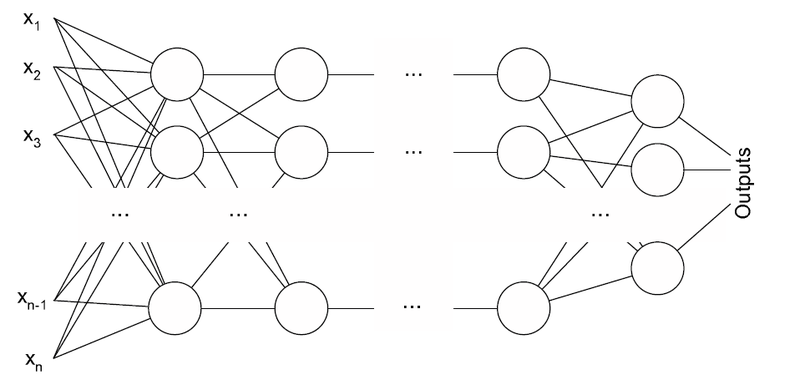
\includegraphics[width=0.65\linewidth]{parceptrone}
			\centering
		\end{figure}
		\subsubsection{Набор гиперпараметров}
		Гиперпарметры многослойного парцептрона Румельхарта, которые будут использованы для оптимизации (в круглых скобках указан тип гиперпараметра, в квадратных -- диапазон его значений):
		\begin{itemize}
			\item hidden layer sizes \textit{(int)} -- число скрытых слоёв [1, 150]
			\item $ \alpha $ \textit{(float)} -- L2 штраф [0.00001, 0.01]
			\item learning rate initial \textit{(float)} -- начальная скорость обучения [0.0001, 0.1]
			\item max iterations \textit{(int)} -- максимальное число итераций [50, 300]
			\item validation fraction \textit{(float)} -- доля данных обучения, отведенных в качестве проверки для преждевременной остановки [0.01, 0.9]
			\item $ \beta_{1} $ \textit{(float)} -- скорость экспоненциального убывания для оценок вектора первого момента [0.09, 0.9]
			\item $ \beta_{2} $ \textit{(float)} -- Скорость экспоненциального убывания для оценок вектора второго момента [0.0999, 0.999]
			\item n iterations no change \textit{(int)} -- максимальное число эпох, пройденных без прогресса [5, 15]
		\end{itemize}
		
		\subsection{Целевая функция}
		Как было упомянуто в части \ref{pr:objf}, целевая функция в нашем случае должна отдавать значение меры качества классификации, вернее обратное её значение, так как идёт процесс минимизации. Поэтому вернёмся к части \ref{s:mcl} и выберем подходящую нам меру оценки качества классификации.\par
		\paragraph{Мера оценки качества классификации} Наиболее подходяей мерой в нашем случае является \textit{F-score}, так как она проста в вычислении и от неё легко берётс обратное значение: \textit{(1 -- F-score)} -- именно это значение будет выдаваться целевой функцией прикаждом обращении к ней.
		Более детально рассмотрим процесс, происходящий внутри целевой функции. До запуска оптимизации, функция инизиализируется выборкой, разделённой на 2 части: \textit{train} и \textit{validate}. Далее запускается оптимизационный процесс, где вызывается наша целевая функция. При каждом обращении, на вход функции подаётся конфигурация гиперпараметров, сгенерированная алгоритмом оптимизации для классификатора. После чего запускается процесс обучения классификатора с заданной конфигурацией на тренировочной части выборки, далее запускается процесс предсказания меток классов на валидационной части выборки, считается значение \textit{F-score} и возвращается описанное ранее значение целевой функции. Затем оптимизатор анализирует полученный результат, перестраивает конфигурацию и повторяет до тех пор, пока не достигнет последней итерации.
	\section{Метрика для определения подобия задач} \label{s:metrics}
	В работе планируется использовать не только априорные знания по решаемой задаче, но и апостериорные знания, полученные при решении других задач. Но так как задач (датасетов) существует бесконечное множество, то возникает вопрос: каким образом выбирать подходящие для нашей задачи и какую информацию из обучения использовать. Фактичести у всех датасетов разное число признаков, классов и радикально разные диапазоны значений. А нам необходимо выяснить не только насколько та или зая задача похожа на решаемую, но и дать количественную оценку подобию задач. в этой части мы рассмотрим меру оценки подобию задач. \par
	Первое, что приходит на ум -- рассчитать расстояние между задачами, однако для рассчёта рассстояний между задачами, необходимо, чтобы задачи имели одинаковую размерность. Для этого их необходимо привести к общему виду. \par 
	Один из способов -- для каждого датасета рассчитать метапризнаки и уже по ним считать расстояния. Для этого для каждого признака возьмём некую характеристику его связи с классом, попарные корреляции между признаками и характеристики структуры дерева принятия решений. После чего на каждом полученном массиве посчитаем статистики (минимум, максимум, среднее и т.д.). полученный массив и будет массивом метапризнаков. Однако этого ещё не достаточно для рассчёта расстояния, так как значения по-прежнему довольно различаются. Поэтому необходимо также нормализовать массивы полученных метапризнаков. После нормализации мы получим не только подходящие значения, но и устраним ковариации и уравним дисперсию.В качестве нормализации используем Расстояние Махалан\'обиса -- это мера расстояния между векторами случайных величин, обобщающая понятие евклидова расстояния. Именно данный подход к нормализации умитывает в себе ковариации. Формально расстояние Махаланобиса он рассматриваемого вектора $ x=(x_{1},x_{2},x_{3}...x_{N})^{T} $ до множества со средним значением $ \mu=(\mu_{1},\mu_{2},\mu_{3}...\mu_{N})^{T} $ матрицей ковариации $ S $ определяется следующим образом:
	\begin{equation}
	\mathit D_{M}(x)=\sqrt{(x-\mu)^{T}S^{-1}(x-\mu)}
	\label{eq:meh}
	\end{equation}\par
	Для удобства изначально домножим на $ S^{-1/2} $, чтобы сокрасить затраны на рассчёт. После того, как мы получим набор нормализованных признаков, посчитаем обыкновенное Евклидово расстояние между задачами:
	\begin{equation}
	\mathit d(p,q)=\sqrt{\sum_{i=1}^{n} (p_{i}-q_{i})^{2}}
	\label{eq:euclid}
	\end{equation}\par
	Теперь для каждой пары задач мы знаем расстояниие между ними и можем использовать это расстояние для оценки подобия задач. Однако в реальности у нас не фиксированный набор задач, постоянно добавляются норые датасеты, а так как нормализация производится по фиксированному множеству задач, то добавление нового датасета может исказить уже посчитанные расстояния и придётся пересчитывать всё с самого начала. Казалось бы это не является универсальным решением, однако если учесть, что предпоститанных задач у нас много больше, чем приходящих (например, имеется 100 предпросчитанных задач и добавляется одна новая), то на значения факт добавления задачи повлияет незначительно и можно почтитать необходимые значения только для новой задачи.
	
	\section{Расширение Байесовской оптимизации}
	В параграфе \ref{pr:bo} описан классический подход к Байесовской оптимизации, цель настоящей работы -- расширить существующий алгоритм до получения лучших результатов при таком же условно временном лимите на обучение. За временной лимит стоит считать количество итераций оптимизатора. Для начала давайте определим, какая информация из соседних задач нам доступна и какая представляет для нас ценность в решении текущей задачи\par
	\subsection{Апостериорная информация} 
	На первом этапе для каждого датасета запустим классическую Байесовскую оптимизацию, на выходе которой получим следующую апостериорную информацию: 
	\begin{itemize}
		\item $ X_{opt} $ -- оптимальная конфигурация гиперпараметров
		\item $ y_{opt} $ -- оптимальное значение целевой функции
		\item $ X $ -- массив рассмотреных конфигураций в порядке итераций
		\item $ y $ -- массив значений целевых функций в порядке итераций
		\item $ incubments $ -- массив оптимальных конфигураций, известных на момент текущей итерации (значение обновляется только в случае получения лучшего результата)
		\item $ incubment_values $ -- массив соответствующих значений целевой функции
		\item $ runtime $ -- массив значений времени, затраченного на соответствующую итерацию (включает в себя время обращения к целевой функции и расчёт значений \textit{incubment})
		\item $ overhead $ -- массив значений времени, затраченного на оптимизацию сверх функции
	\end{itemize}
	Значения \textit{runtime} и \textit{overhead} могут быть полезны для оценки времени работы модифицированного алгоритма. По значениям \textit{incubment values} можно оценить на каких итерациях мы получаем улучшения, а значения оптимальных конфигураций использовать как полезную нам апостериорную информацию для решаемой задачи. \par 
	Рассмотрим наглядный пример, что происходит на каждой итерации. На рисунке \ref{img:bogp} представлен пример Байесовской оптимизации на основе гауссовского процесса. В качестве примера взята одномерная функция для упрощения понимания. Точки на графике определяют гиперпараметры, в данном случае гиперпараметр. 
	\begin{figure}[!ht]
		\caption{Пример Байесовской оптимизации на основе Гауссовского процесса для одномерной функции.}\label{img:bogp}
		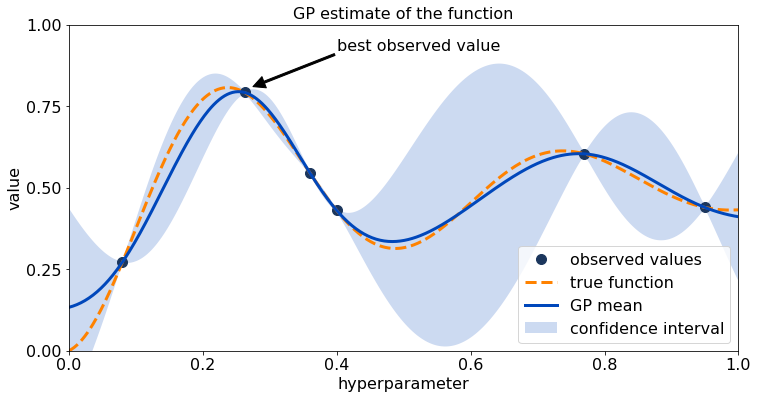
\includegraphics[width=0.85\linewidth]{bo_gp}
		\centering
	\end{figure}
	Оранжевой пунктирной линией показано настоящее значение функции <<чёрного>> ящика, которое на самом деле нам не известно, онако мы пытаемся с течением каждой итерации оптимизации приблизиться к её значению. Как уже говорилось, на каждой итерации мы получаем значение целевой функции (это и есть наша функция <<чёрного ящика>>) и всё больше приближаемся к действительному значению. \par
	Для старта модели необходимо иметь 3 точки, чтобы понимать, от чего отталкиваться в ходе решения. В общем случае эти точки задаются случайно, как говорилось в главе \ref{chp1}, однако в нашем случае мы знаем результаты обучения на подобных задачах, а также меру подобия задач и можем расставить начальные точки не случайно.
	\subsection{Расстановка начальных конфигураций}
	Так как для старта модели необходимо 3 точки, имеет смысл рассмотреть 3 ближайшие задачи и получить оптимальный набоор гиперпараметров от каждой. Сам по такой подход уже может дать приемущество перед случайной расстановкой, однако этого не достаточно для получения иновационного результата. Кроме того мы обладаем пполной иформацией об обучении соседних задач, что можно использовать. \par 
	Для начала давайте определим понятие \textit{достоверности (reliability)}, которое будет показывать, на сколько можно <<доверять>> апостериорным знаниям той или иной задачи. Посчитанное в части \ref{s:metrics} значение расстояния было бы использовать некорректно как минимум по причине того, что оно не нормализовано для модели оптимизации и значения могут значительно именятся с добавлением новых задач и пересчётом метрики. Поэтому введём следующее определение достоверности:
	\begin{equation}
	\mathit R^{t}=(\alpha^{t}-K(d_{1})+(1-\alpha^{t})K(\zeta_{1}))
	\label{eq:rel}
	\end{equation}
	%% TODO картиночки
	где $ t $ -- номер итерации оптимизатора, $ \alpha $ -- мера <<забывания>> апостериорной информации (от 0 до 1), $ d_{1} $ -- расстояние до задачи 1, $ \zeta_{1} $ -- гобальная мера, на сколько обличается конфигурация задачи 1 от решаемой, $ K(d_{1}), K(\zeta_{1})$ -- функции ядра. \par 
	Так как диапазоны значений для каждого гимерпараметра могут существенно отличатся, то нас интересует не только глобальное значение параметра $ \zeta $, но и его полная его характеристика для каждой задачи (то есть на сколько отличается каждое из значений гиперпараметров). Формально у нас для каждой задачи (относительно решаемой) будет считаться 2 характиристики: гобальное число и локальный массив. Связаны эти значения следующим образом: 
	\begin{equation}
	\mathit \zeta_{local} = \{\Delta x_{1}, \Delta x_{2}...\Delta x_{N}\}, \zeta_{global} = \mathrm{avg}_{i}(\Delta x_{i})
	\label{eq:zeta}
	\end{equation}
	где avg -- среднее значение.
	
	\chapterconclusion
	В данной главе было описано предложенное решение по улучшению Байесовской оптимизации. В качестве метрики для определения подобия задач предложено Евклидово расстояние, рассчитанное на нормализованных метапризнаках по всем датасетам. В качестве меры доставерности информации об обучении предложена собственная мера, которая основывается на ядерной функции от расстояни до датасета и разница по каждому гиперпараметру в корфигурации.
	
	\chapter{Анализ полученных результатов}
	Полный список результатов классической Байесовской оптимизации можно найти в приложении  \ref{sec:app:1}.
	\begin{figure}[!ht]
		\caption{Результат классической Байесовской оптимизации для задачи car}\label{img:bo}
		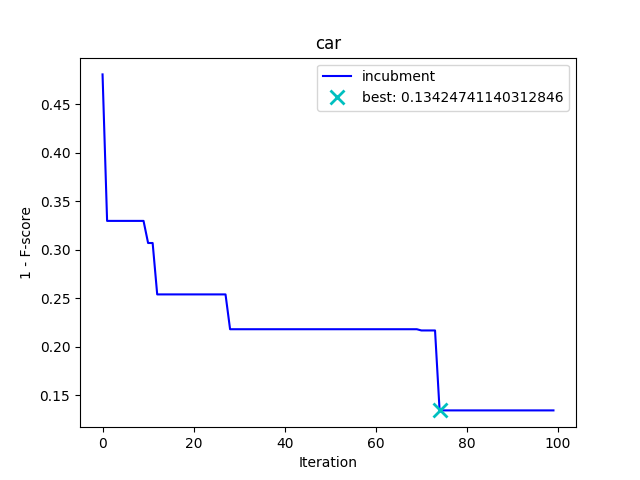
\includegraphics[width=0.85\linewidth]{car}
		\centering
	\end{figure}
	\begin{figure}[!ht]
	\caption{Результат классической Байесовской оптимизации для задачи glass}\label{img:bo}
	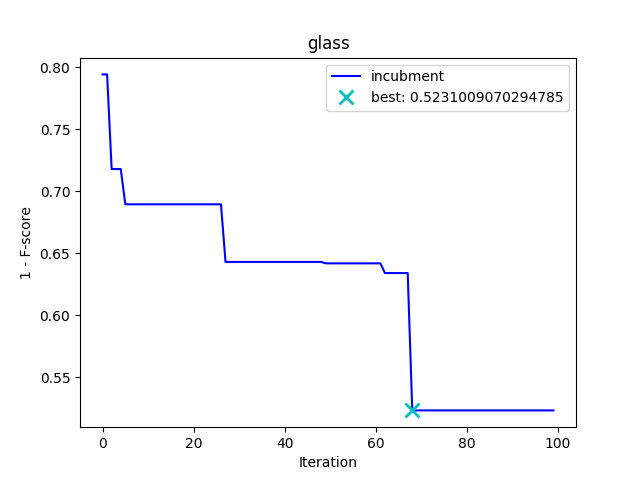
\includegraphics[width=0.85\linewidth]{glass}
	\centering
\end{figure}
	\begin{figure}[!ht]
	\caption{Результат классической Байесовской оптимизации для задачи wine}\label{img:bo}
	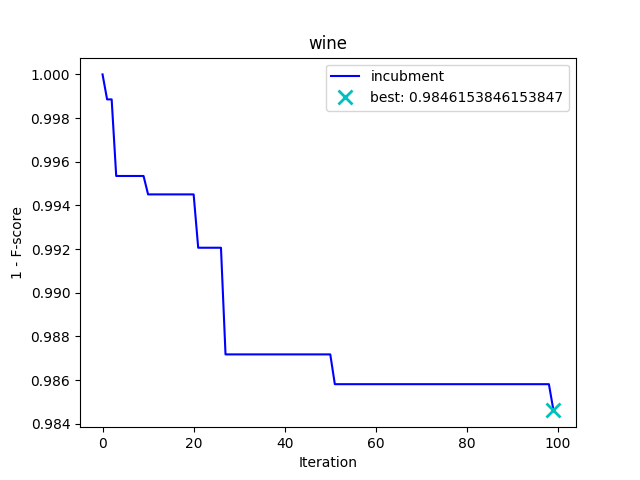
\includegraphics[width=0.85\linewidth]{wine}
	\centering
\end{figure}

Полный список результатов предложенной Байесовской оптимизации можно найти в приложении  \ref{sec:app:2}.
	\begin{figure}[!ht]
	\caption{Результат предложенной Байесовской оптимизации для задачи car}\label{img:bo}
	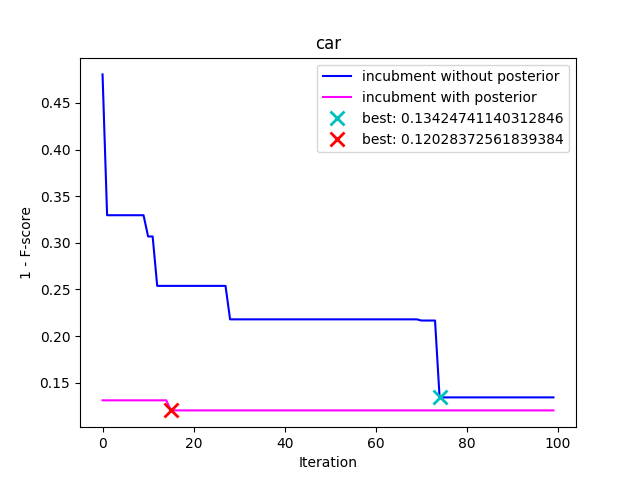
\includegraphics[width=0.85\linewidth]{p-car}
	\centering
\end{figure}
\begin{figure}[!ht]
	\caption{Результат предложенной Байесовской оптимизации для задачи glass}\label{img:bo}
	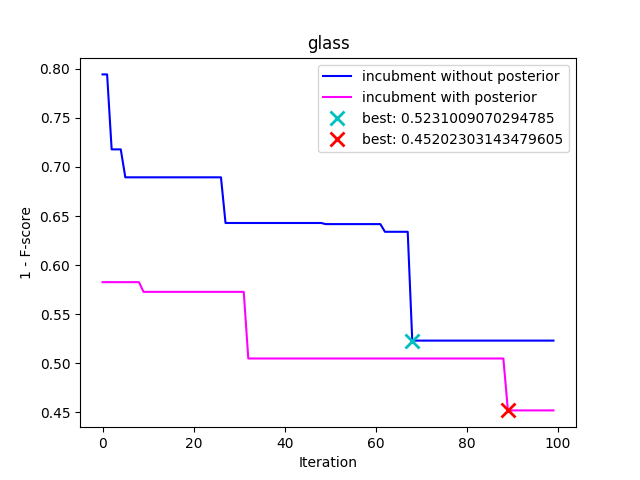
\includegraphics[width=0.85\linewidth]{p-glass}
	\centering
\end{figure}
\begin{figure}[!ht]
	\caption{Результат предложенной Байесовской оптимизации для задачи wine}\label{img:bo}
	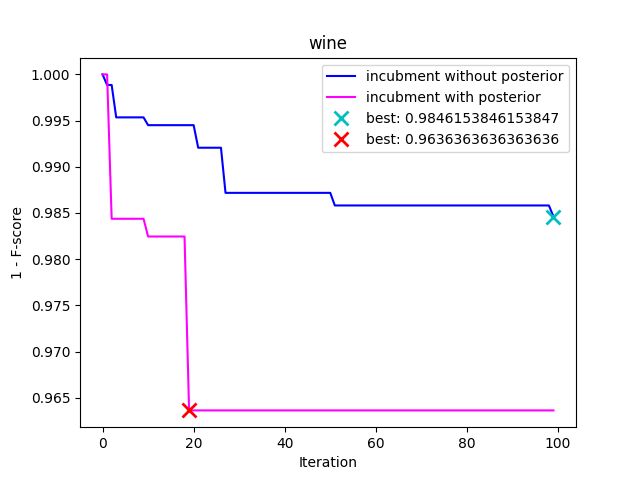
\includegraphics[width=0.85\linewidth]{p-wine}
	\centering
\end{figure}

	\chapterconclusion
	По результатам видно, что предложенный алгоритм работает эффективнее классической Байесовской оптимизации.
	
	
	%% Макрос для заключения. Совместим со старым стилевиком.
	\startconclusionpage
	В ходе исследования были рассмотрены существующие решения для проблемы оптимизации гиперпараметров и предложено новое эффективное решение, которое показало свою эффективность на статистических экспериментах.
	
	\printmainbibliography
	
	
	%% После этой команды chapter будет генерировать приложения, нумерованные русскими буквами.
	%% \startappendices из старого стилевика будет делать то же самое
	\appendix
	\chapter{Результаты классической Байесовской оптимизации}\label{sec:app:1}
	\begin{center}
		\begin{longtable}{ |m{5cm}|c|c| } 
			\hline
			\textbf{Имя датасета} & \textbf{Лучшее значение (1 - F-score)} & \textbf{Номер итерации} \\ 
			\hline\hline
			page-blocks & 0.1572831335432724 & 42 \\
			\hline
			robot-failures-lp1 & 0.14102564102564108 & 33 \\
			\hline
			mfeat-fourier & 0.1475854394148598 & 2 \\
			\hline
			jungle-chess-2pcs-raw-endgame-complete & 0.2719523672987666 & 27 \\
			\hline
			heart-switzerland & 0.6858119658119658 & 91 \\
			\hline
			gas-drift-different-concentrations & 0.01891421038359764 & 77 \\
			\hline
			wall-robot-navigation & 0.01529599728237685 & 57 \\
			\hline
			jungle-chess-2pcs-endgame-panther-elephant & 0.0 & 88 \\
			\hline
			leaf & 0.36017355660212813 & 73 \\
			\hline
			PopularKids & 0.06352989828599576 & 40 \\
			\hline
			mfeat-karhunen & 0.014079861405182248 & 20 \\
			\hline
			diggle-table-a2 & 0.9743589743589743 & 84 \\
			\hline
			rmftsa-sleepdata & 0.9278268809884568 & 27 \\
			\hline
			semeion & 0.05376620700232804 & 28 \\
			\hline
			desharnais & 0.2667332667332668 & 86 \\
			\hline
			teachingAssistant & 0.4071969696969696 & 44 \\
			\hline
			collins & 0.8884880528144286 & 38 \\
			\hline
			volcanoes-a3 & 0.7689402697495183 & 61 \\
			\hline
			artificial-characters & 0.3613704595813323 & 30 \\
			\hline
			volcanoes-a4 & 0.7972789115646258 & 51 \\
			\hline
			glass & 0.5231009070294785 & 68 \\
			\hline
			nursery & 0.04052981019439761 & 61 \\
			\hline
			shuttle & 0.0 & 30 \\
			\hline
			segment & 0.02531199490574576 & 62 \\
			\hline
			heart-long-beach & 0.652975912975913 & 91 \\
			\hline
			vertebra-column & 0.20623124372223145 & 80 \\
			\hline
			cnae-9 & 0.034818671429924564 & 26 \\
			\hline
			jannis & 0.9999969017034435 & 10 \\
			\hline
			wine-quality-white & 0.750911817087637 & 40 \\
			\hline
			vehicle & 0.34988621629488503 & 36 \\
			\hline
			ecoli & 0.24709595959595954 & 58 \\
			\hline
			eye-movements & 0.5769399013962551 & 16 \\
			\hline
			seeds & 0.11004901960784308 & 96 \\
			\hline
			car & 0.13424741140312846 & 74 \\
			\hline
			fabert & 0.8754012841091493 & 0 \\
			\hline
			breast-tissue & 0.6674242424242425 & 64 \\
			\hline
			thyroid-allbp & 0.5548263021310648 & 81 \\
			\hline
			gas-drift & 0.011142829995818726 & 81 \\
			\hline
			mfeat-factors & 0.08802270506646293 & 53 \\
			\hline
			volcanoes-d1 & 0.7974875207986689 & 10 \\
			\hline
			har & 0.013956849985395814 & 39 \\
			\hline
			satimage & 0.10895145985989307 & 73 \\
			\hline
			Fashion-MNIST & 0.1732567305672541 & 47 \\
			\hline
			seismic-bumps & 0.03781821523757012 & 34 \\
			\hline
			pokerhand & 0.28102343233242333 & 84 \\
			\hline
			helena & 0.981850107656847 & 98 \\
			\hline
			thyroid-allhyper & 0.5208075903466287 & 14 \\
			\hline
			wine & 0.9846153846153847 & 99 \\
			\hline
			balance-scale & 0.07249605495219524 & 46 \\
			\hline
			microaggregation2 & 0.5627566824728257 & 44 \\
			\hline
			steel-plates-fault & 0.7677201034057892 & 61 \\
			\hline
			tae & 0.3234408602150539 & 22 \\
			\hline
			mfeat-pixel & 0.5312663695353331 & 92 \\
			\hline
			gina-prior2 & 0.08624343753649555 & 81 \\
			\hline
			synthetic-control & 0.0 & 7 \\
			\hline
			cmc & 0.4217043857598791 & 12 \\
			\hline
			energy-efficiency & 0.8637585814858542 & 22 \\
			\hline
			iris & 0.0 & 2 \\
			\hline
			fars & 0.4350632170299382 & 22 \\
			\hline
			abalone & 0.6296727096012757 & 95 \\
			\hline
			prnn-viruses & 0.0 & 62 \\
			\hline
			Indian-pines & 0.5687291627863662 & 4 \\
			\hline
			covertype & 0.4420032958440877 & 5 \\
			\hline
			JapaneseVowels & 0.44703798338069056 & 91 \\
			\hline
			user-knowledge & 0.1050103519668737 & 29 \\
			\hline
			spectrometer & 0.9662337662337662 & 47 \\
			\hline
			hayes-roth & 0.12222222222222212 & 34 \\
			\hline
			robot-failures-lp5 & 0.2971834250941756 & 59 \\
			\hline
			prnn-fglass & 0.3836808236808237 & 27 \\
			\hline
			waveform-5000 & 0.12700439195696356 & 27 \\
			\hline
			zoo & 0.0 & 12 \\
			\hline
			cardiotocography & 0.06492996280208396 & 96 \\
			\hline
			mfeat-morphological & 0.5482421206646882 & 6 \\
			\hline
			volcanoes-a1 & 0.8019336485603352 & 98 \\
			\hline
			tamilnadu-electricity & 0.0755314544908181 & 40 \\
			\hline
			LED-display-domain-7digit & 0.21607382867705938 & 44 \\
			\hline 
			
		\end{longtable}
	\end{center}

	\chapter{Результаты классической Байесовской оптимизации}\label{sec:app:1}
	\begin{center}
		\begin{longtable}{ |m{3.4cm}|m{4.7cm}|m{4.7cm}|m{1.5cm}|m{1.5cm}| } 
		\hline
		\textbf{Имя датасета} & \textbf{Лучшее значение (1 - F-score) (КБО)} & \textbf{Лучшее значение (1 - F-score) (ПБО)} & \textbf{Номер итерации (КБО)} &  \textbf{Номер итерации (ПБО)} \\
		\hline\hline
		car & 0.13424741140312846 & 0.12028372561839384 & 74 & 15 \\
		\hline
		wine & 0.9846153846153847 & 0.9636363636363636 & 99 & 19 \\
		\hline
		cmc & 0.4217043857598791 & 0.4608957535597932 & 12 & 89 \\
		\hline
		zoo & 0.0 & 0.0 & 12 & 11 \\
		\hline
		nursery & 0.04052981019439761 & 0.05928043944850669 & 61 & 63 \\
		\hline
		abalone & 0.6296727096012757 & 0.629497094309903 & 95 & 12 \\
		\hline
		cardiotocography & 0.06492996280208396 & 0.06644365589389312 & 96 & 57 \\
		\hline
		desharnais & 0.2667332667332668 & 0.261437908496732 & 86 & 84 \\
		\hline
		glass & 0.5231009070294785 & 0.45202303143479605 & 68 & 89 \\
		\hline
		segment & 0.02531199490574576 & 0.03319329454434661 & 62 & 22 \\
		\hline
		
		\end{longtable}
	\end{center}
\end{document}